\documentclass{beamer}

% \usepackage{beamerthemesplit} // Activate for custom appearance

\usepackage{inputenc}
\usepackage[english]{babel}
\usepackage{graphicx}
\usepackage[compatibility=false]{caption}
\usepackage{subcaption}
\usepackage{tikz}
\usepackage{ragged2e}
%\usepackage{freetikz}
\usepackage{comment}
\usepackage{mathtools, braket}

\usepackage{color}

%\usepackage{pgfpages}
%\pgfpagesuselayout{2 on 1}[a4paper,border shrink=5mm]

\usepackage{amsmath}
\usepackage{amssymb}
\usepackage{amsfonts}

\usepackage{csquotes}

\usepackage[T1]{fontenc}

\setbeamertemplate{footline}[frame number]
\graphicspath{ {images/} }

%\newtheorem{theorem}[equation]{Theorem}
\newtheorem{claim}[equation]{Claim}
\newtheorem{proposition}[equation]{Proposition}
%\newtheorem{lemma}[equation]{Lemma}
%\newtheorem{corollary}[equation]{Corollary}
\newtheorem{conjecture}[equation]{Conjecture}
%\newtheorem{problem}[equation]{Problem}
\newtheorem{question}[equation]{Question}
\newtheorem{construction}[equation]{Construction}

\theoremstyle{definition}
%\newtheorem{example}[equation]{Example}
%\newtheorem{definition}[equation]{Definition}

\newtheorem{remark}[equation]{Remark}

\newcommand{\changefont}[3]{\fontfamily{#1} \fontseries{#2} \fontshape{#3} \selectfont}

\newcommand{\op}[1]{\ensuremath \mathcal{O}(#1)} %cat of open sets of a topo space
%\newcommand{\Set}{\ensuremath \mathbf{Set}}
\newcommand{\Top}{\ensuremath \mathbf{Top}}
\newcommand{\Bund}{\ensuremath \mathbf{Bund}}
\newcommand{\PSh}{\ensuremath \mathbf{PSh}}
\newcommand{\Sh}{\ensuremath \mathbf{Sh}}
\newcommand{\Et}{\ensuremath \mathbf{Et}}
\newcommand{\cat}[1]{\ensuremath \mathcal{#1}}
\newcommand{\R}{\ensuremath \mathbb R}
\newcommand{\N}{\ensuremath \mathbb N}
\newcommand{\id}{\mathbin{\textrm{\normalfont id}}} % non-italic identity in math mode

\newcommand{\monoid}[1]
{
	\resizebox{#1}{!}{
    \begin{tikzpicture}
		\node[dot,fill=black] (d0) at (3.5, 5.5) {};
		\draw (d0.center) to[out=180, in=90] (3, 4.5);
		\draw (d0.center) to[out=0, in=90] (4, 4.5);
		\draw (d0.center) to[out=90, in=-90] (3.5, 6.5);
    \end{tikzpicture}
	}
}

\newcommand{\unit}[1]
{
	\resizebox{#1}{!}{
    \begin{tikzpicture}
		\node[dot,fill=black] (d0) at (4, 4) {};
		\draw (d0.center) to[out=90, in=-90] (4, 5);
    \end{tikzpicture}
	}
}

\newcommand{\monoidW}[1]
{
	\resizebox{#1}{!}{
    \begin{tikzpicture}
		\node[dot,fill=white] (d0) at (3.5, 5.5) {};
		\draw (d0.center) to[out=180, in=90] (3, 4.5);
		\draw (d0.center) to[out=0, in=90] (4, 4.5);
		\draw (d0.center) to[out=90, in=-90] (3.5, 6.5);
    \end{tikzpicture}
	}
}

\newcommand{\unitW}[1]
{
	\resizebox{#1}{!}{
    \begin{tikzpicture}
		\node[dot,fill=white] (d0) at (4, 4) {};
		\draw (d0.center) to[out=90, in=-90] (4, 5);
    \end{tikzpicture}
	}
}

\newcommand{\comonoid}[1]{\rotatebox[origin=c]{180}{\monoidW{#1}}}
\newcommand{\counit}[1]{\rotatebox[origin=c]{180}{\unitW{#1}}}


\begin{document}

\setbeamertemplate{navigation symbols}{}

\changefont{cmss}{m}{n}
\title{A Finite Presentation of CNOT-dihedral Operators}
\author{Matthew Amy, Jianxin Chen, Neil J. Ross}
\date{}
\frame{\titlepage}


\frame{\frametitle{Outline}\tableofcontents}

\section{Quantum circuits}

\begin{frame}{Classical circuits}
	\begin{itemize}
		\item Logical gates (boolean functions $\mathbb{B}^n \rightarrow \mathbb{B}^m$):
		\begin{figure}
		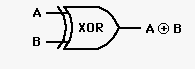
\includegraphics[width=4cm]{images/IMG-XOR}
		\centering
		\end{figure}
		\item Reversible gates (information is physical):
		\begin{figure}
		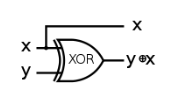
\includegraphics[width=4cm]{images/IMG-revXOR}
		\centering
		\end{figure}
	\end{itemize}
\end{frame}

\begin{frame}{Quantum circuits}
	\begin{itemize}
		\item Logical gates (linear maps $(\mathbb{CB})^n \rightarrow (\mathbb{CB})^m$):
		\begin{figure}
		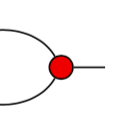
\includegraphics[width=2.6cm]{images/IMG-redspider}
		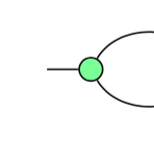
\includegraphics[width=3.2cm]{images/IMG-greenspider}
		\centering
		\end{figure}
		\item Reversible gates (unitaries):
		\begin{figure}
		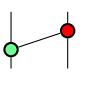
\includegraphics[angle=-90, width=3cm]{images/IMG-CNOT}
		\centering
		\end{figure}
	\end{itemize}
\end{frame}


\section{Clifford+T and universal gate sets}
\begin{frame}{Towards an algebraic theory of quantum circuits}
	Axiomatisations of logical gates (linear maps): ZX, ZW.\\
	Clifford+T is a universal set of (unitary) gates for quantum computing, generated by $\{CNOT, X, H, T \}$.\\
	Want an algebraic theory of reversible (unitary) quantum circuits.
	\begin{itemize}
		\item Lafont (2003): classical case + affine quantum circuits $\{ CNOT, X \}$,
		\item Selinger (2015): generators and relations for the Clifford groupoid $\{ CNOT, X, H, T^2\}$,
		\item Amy et al. (2016): phase polynomials, T-count optimization $\{ CNOT, T\}$,
		\item The present paper gives generators and relations for CNOT-dihedral groupoid $\{CNOT, X, T\}$.
	\end{itemize}
\end{frame}

\section{CNOT-dihedral gates}

\begin{frame}{CNOT-dihedral gates}

In the paper, the CNOT-dihedral operators are defined as follows.
\begin{figure}
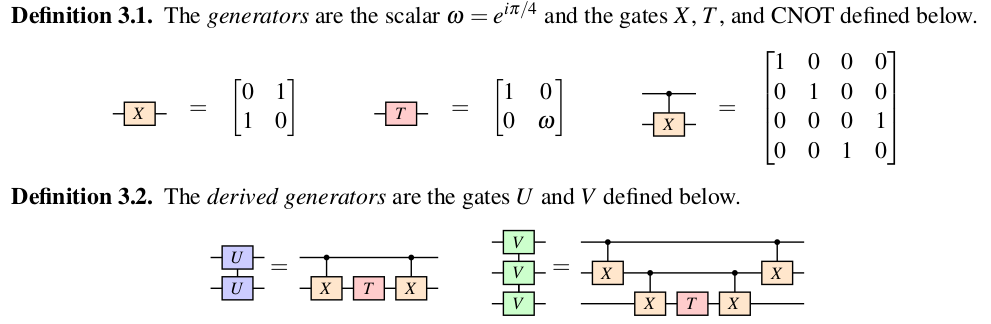
\includegraphics[width=10cm]{gates}
\centering
\caption{Amy, Chen and Ross, p.~86.}
\end{figure}
\begin{itemize}
\item The gates $X$, $CNOT$ and $SWAP$ are called {\em affine}.
\item The gates $\omega$, $T$, $U$ and $V$ are called {\em diagonal}.
\end{itemize}
\end{frame}

\begin{frame}{CNOT-dihedral gates in ZX}

The gates can be expressed in the ZX-calculus.
\begin{figure}
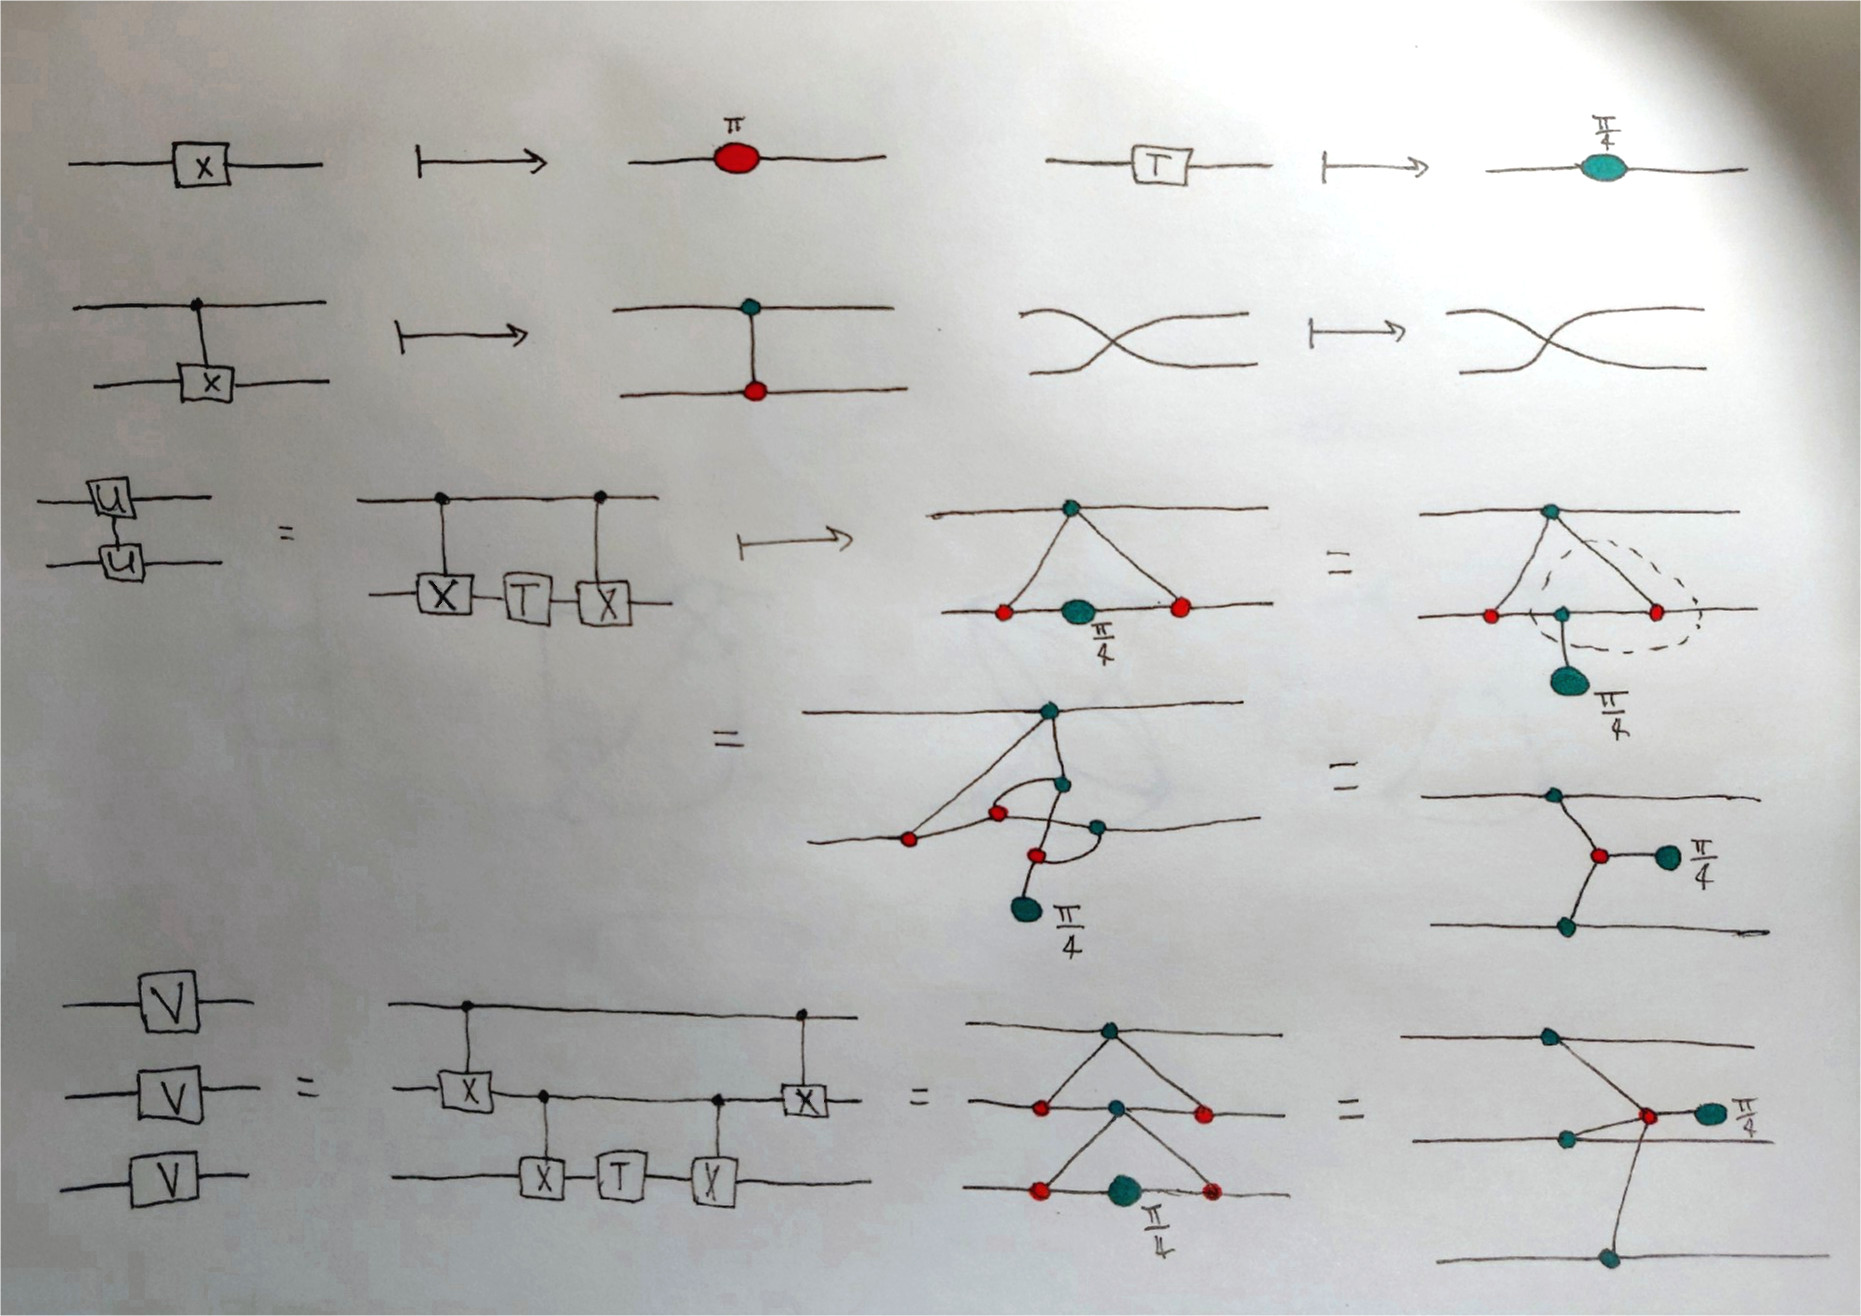
\includegraphics[width=10cm]{gates-in-ZX}
\centering
\end{figure}
\begin{figure}
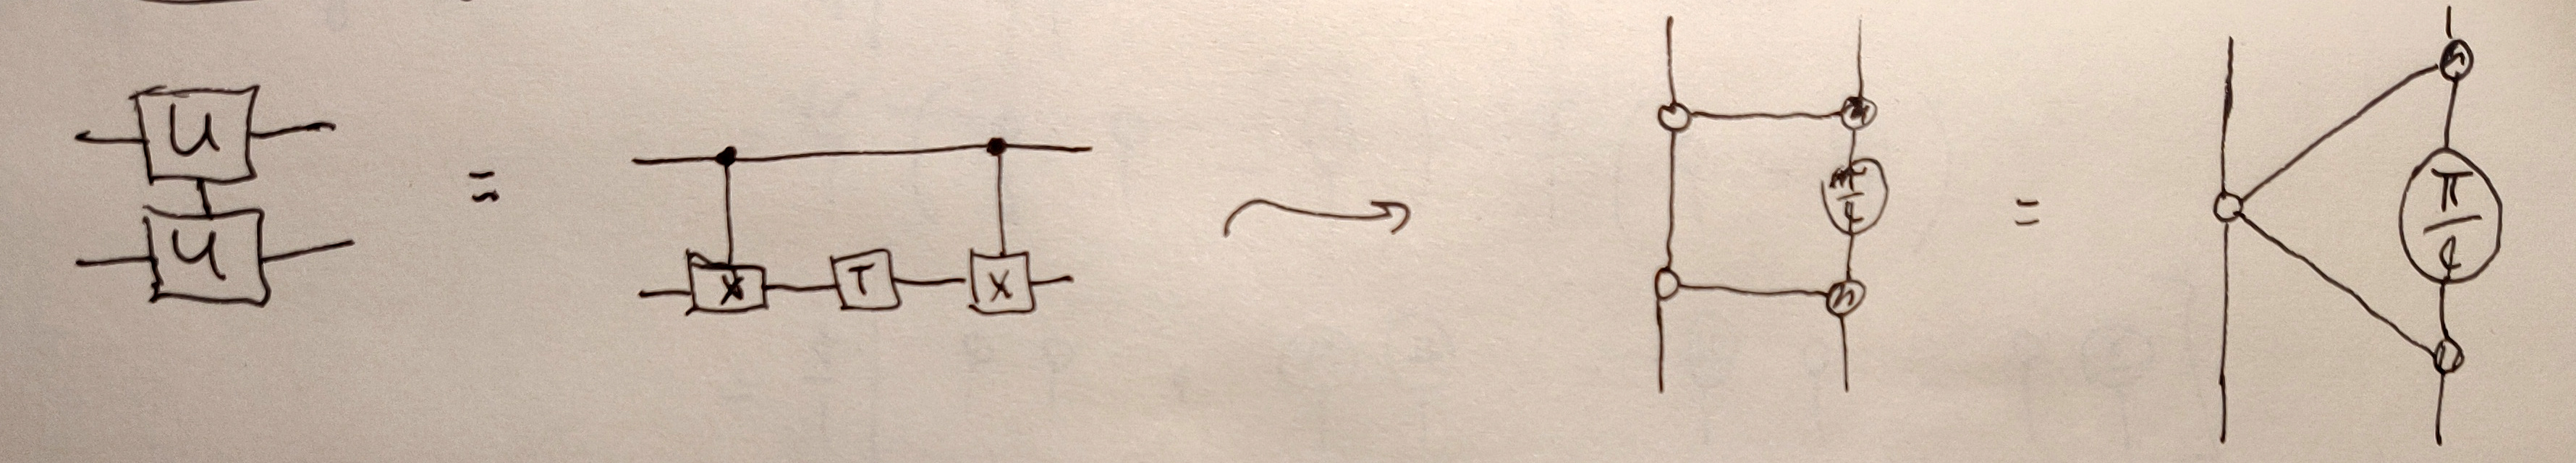
\includegraphics[width=10cm]{U-in-ZX}
\centering
\end{figure}
\end{frame}

\begin{frame}{CNOT-dihedral gates in ZX}
\begin{figure}
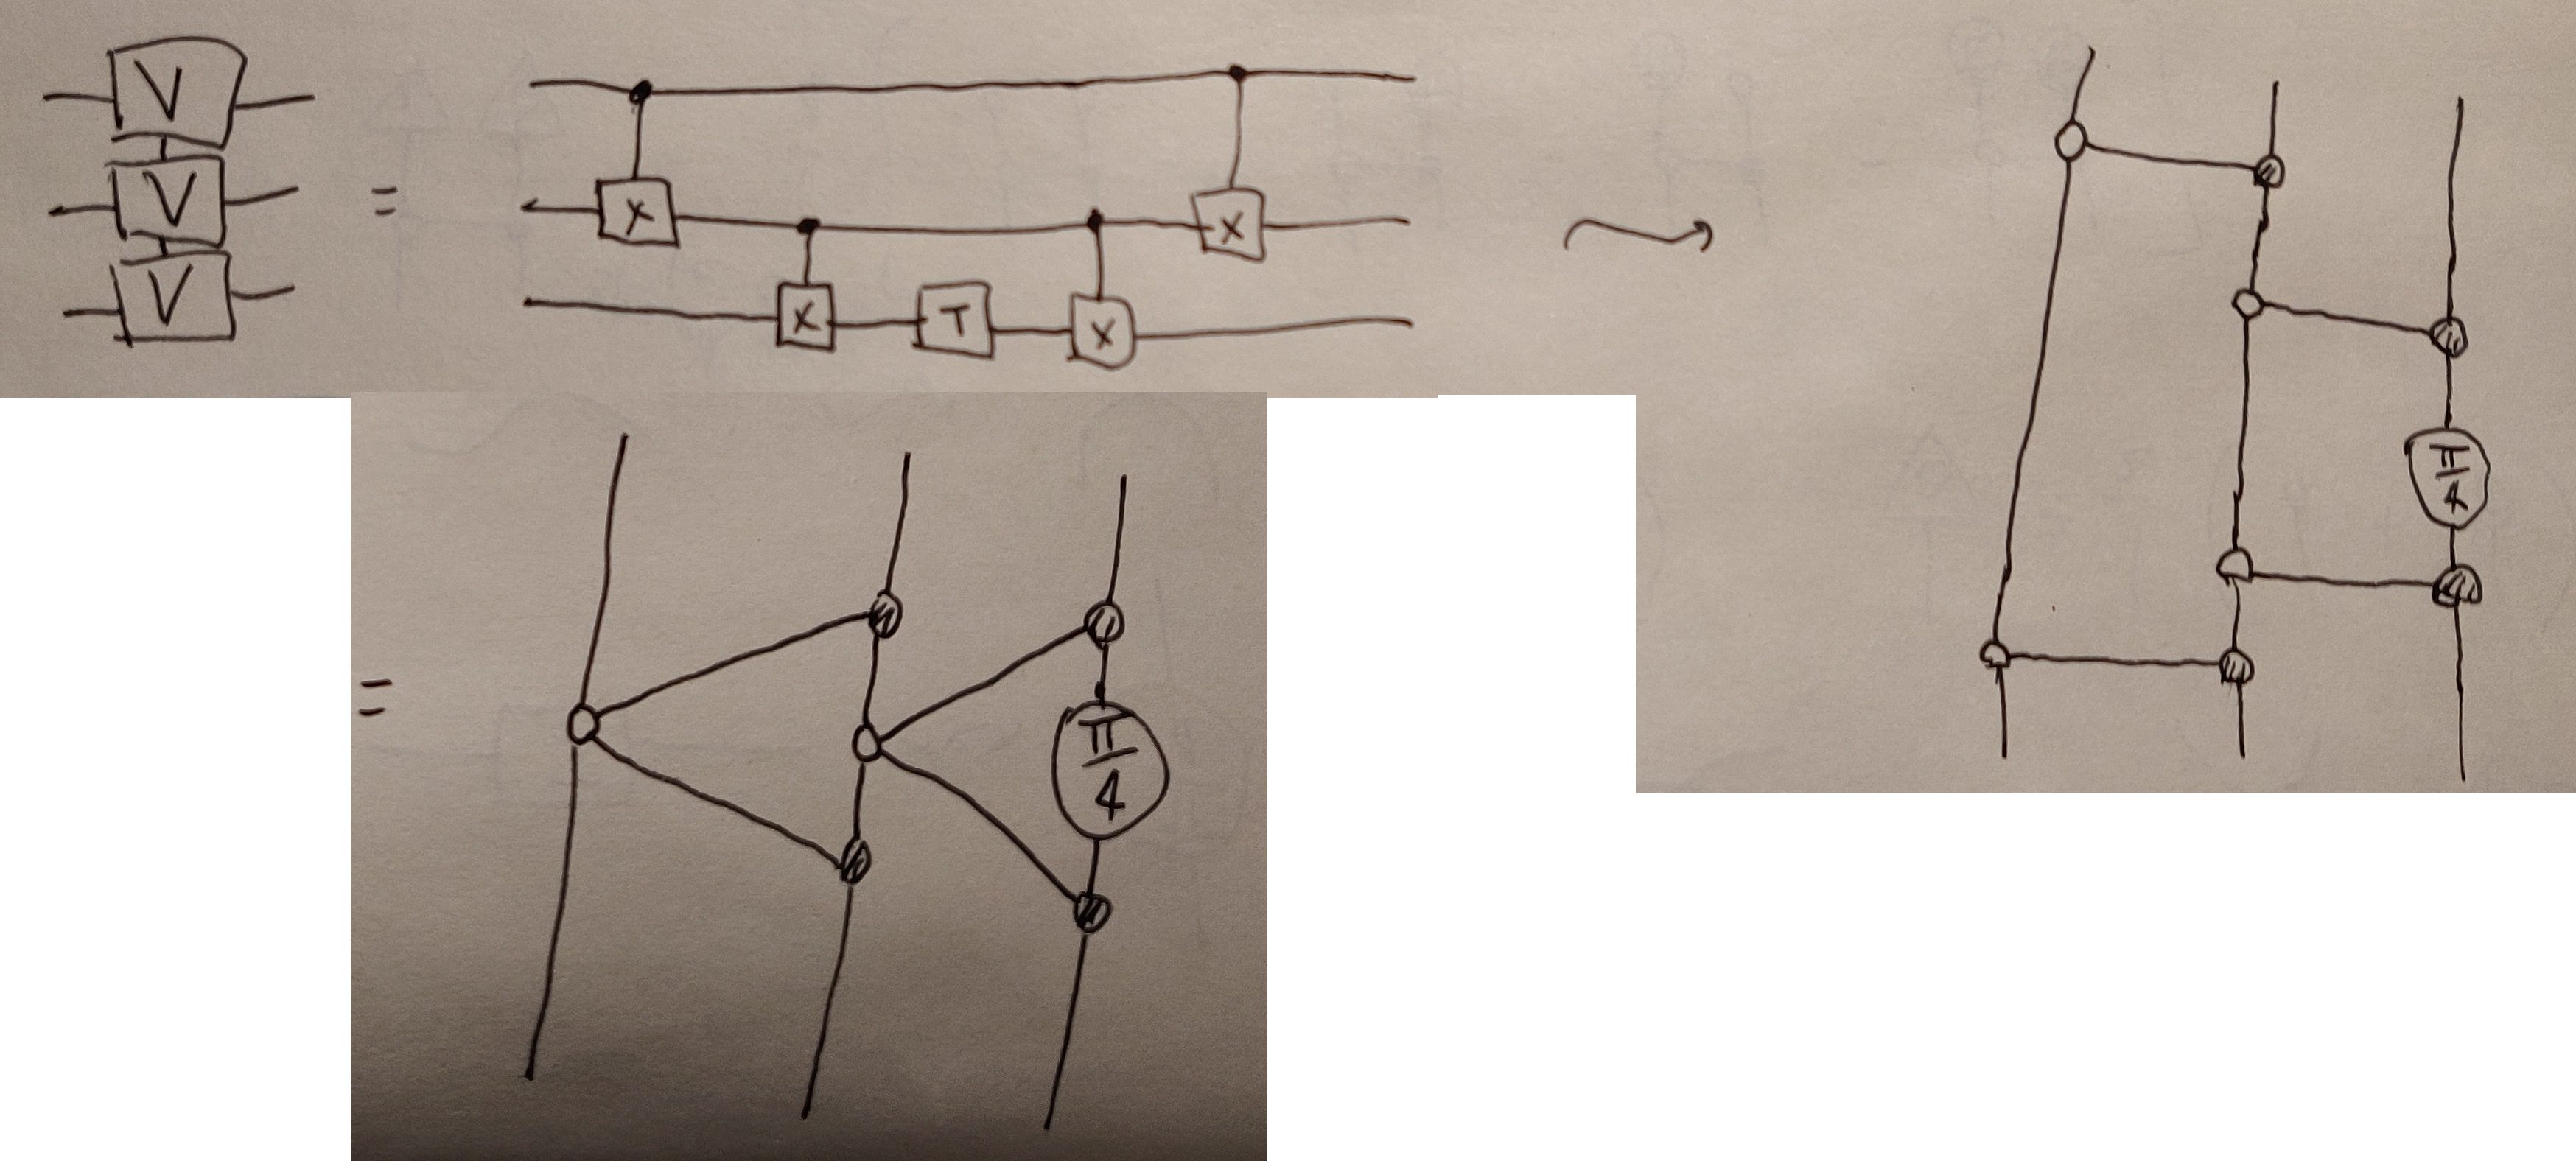
\includegraphics[width=11cm]{V-in-ZX}
\centering
\end{figure}
\end{frame}

\section{Rules for CNOT-dihedral gates}

\begin{frame}{Rules for CNOT-dihedral gates}

\begin{figure}
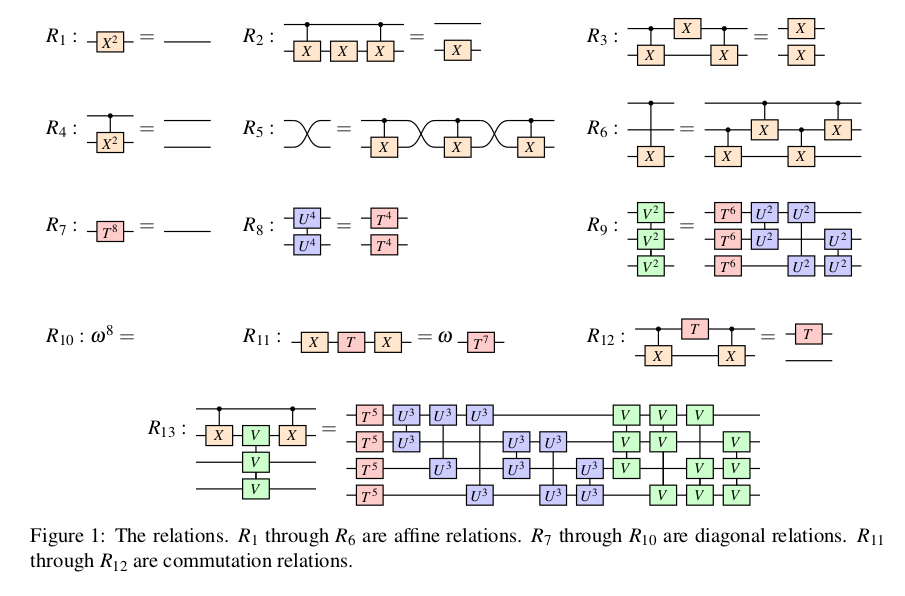
\includegraphics[width=10cm]{relations}
\centering
\caption{Amy, Chen and Ross, p.~87.}
\end{figure}
\end{frame}

\begin{frame}{Derivation of R3 ZX}

\begin{figure}
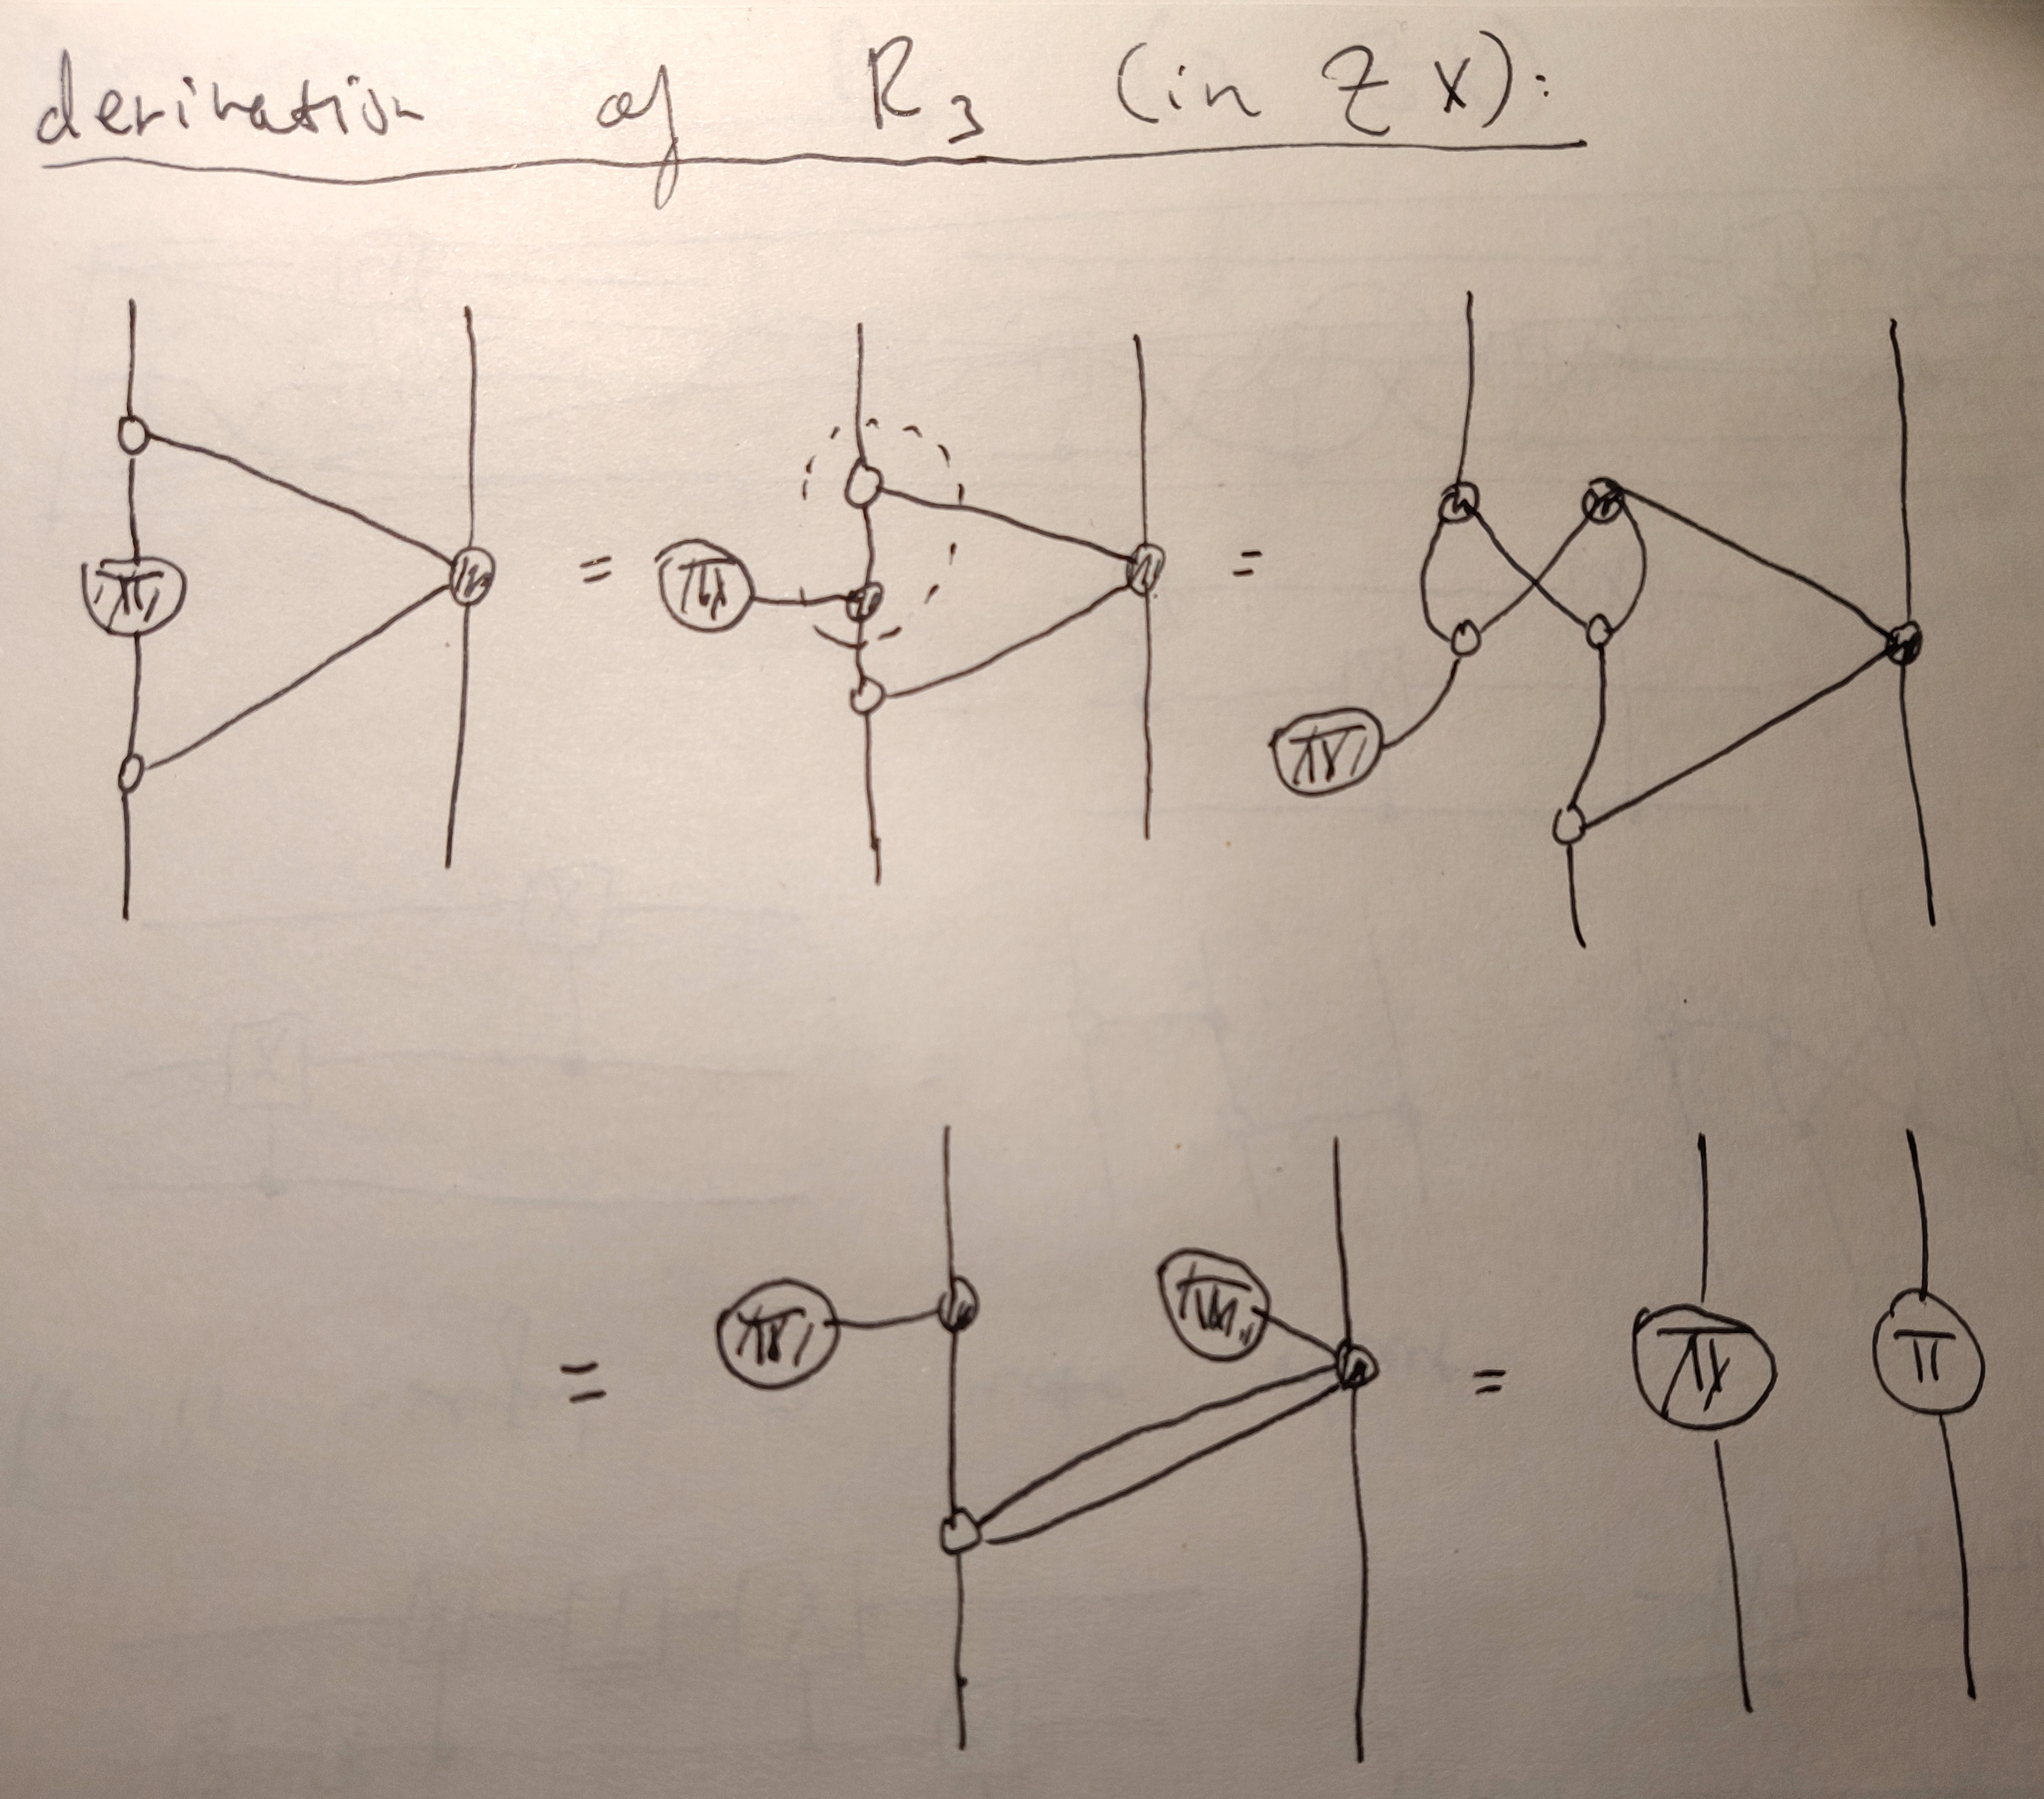
\includegraphics[width=9cm]{R3}
\centering
\end{figure}
\end{frame}

\begin{frame}{Derivation of R5 and R6 in ZX}

\begin{figure}
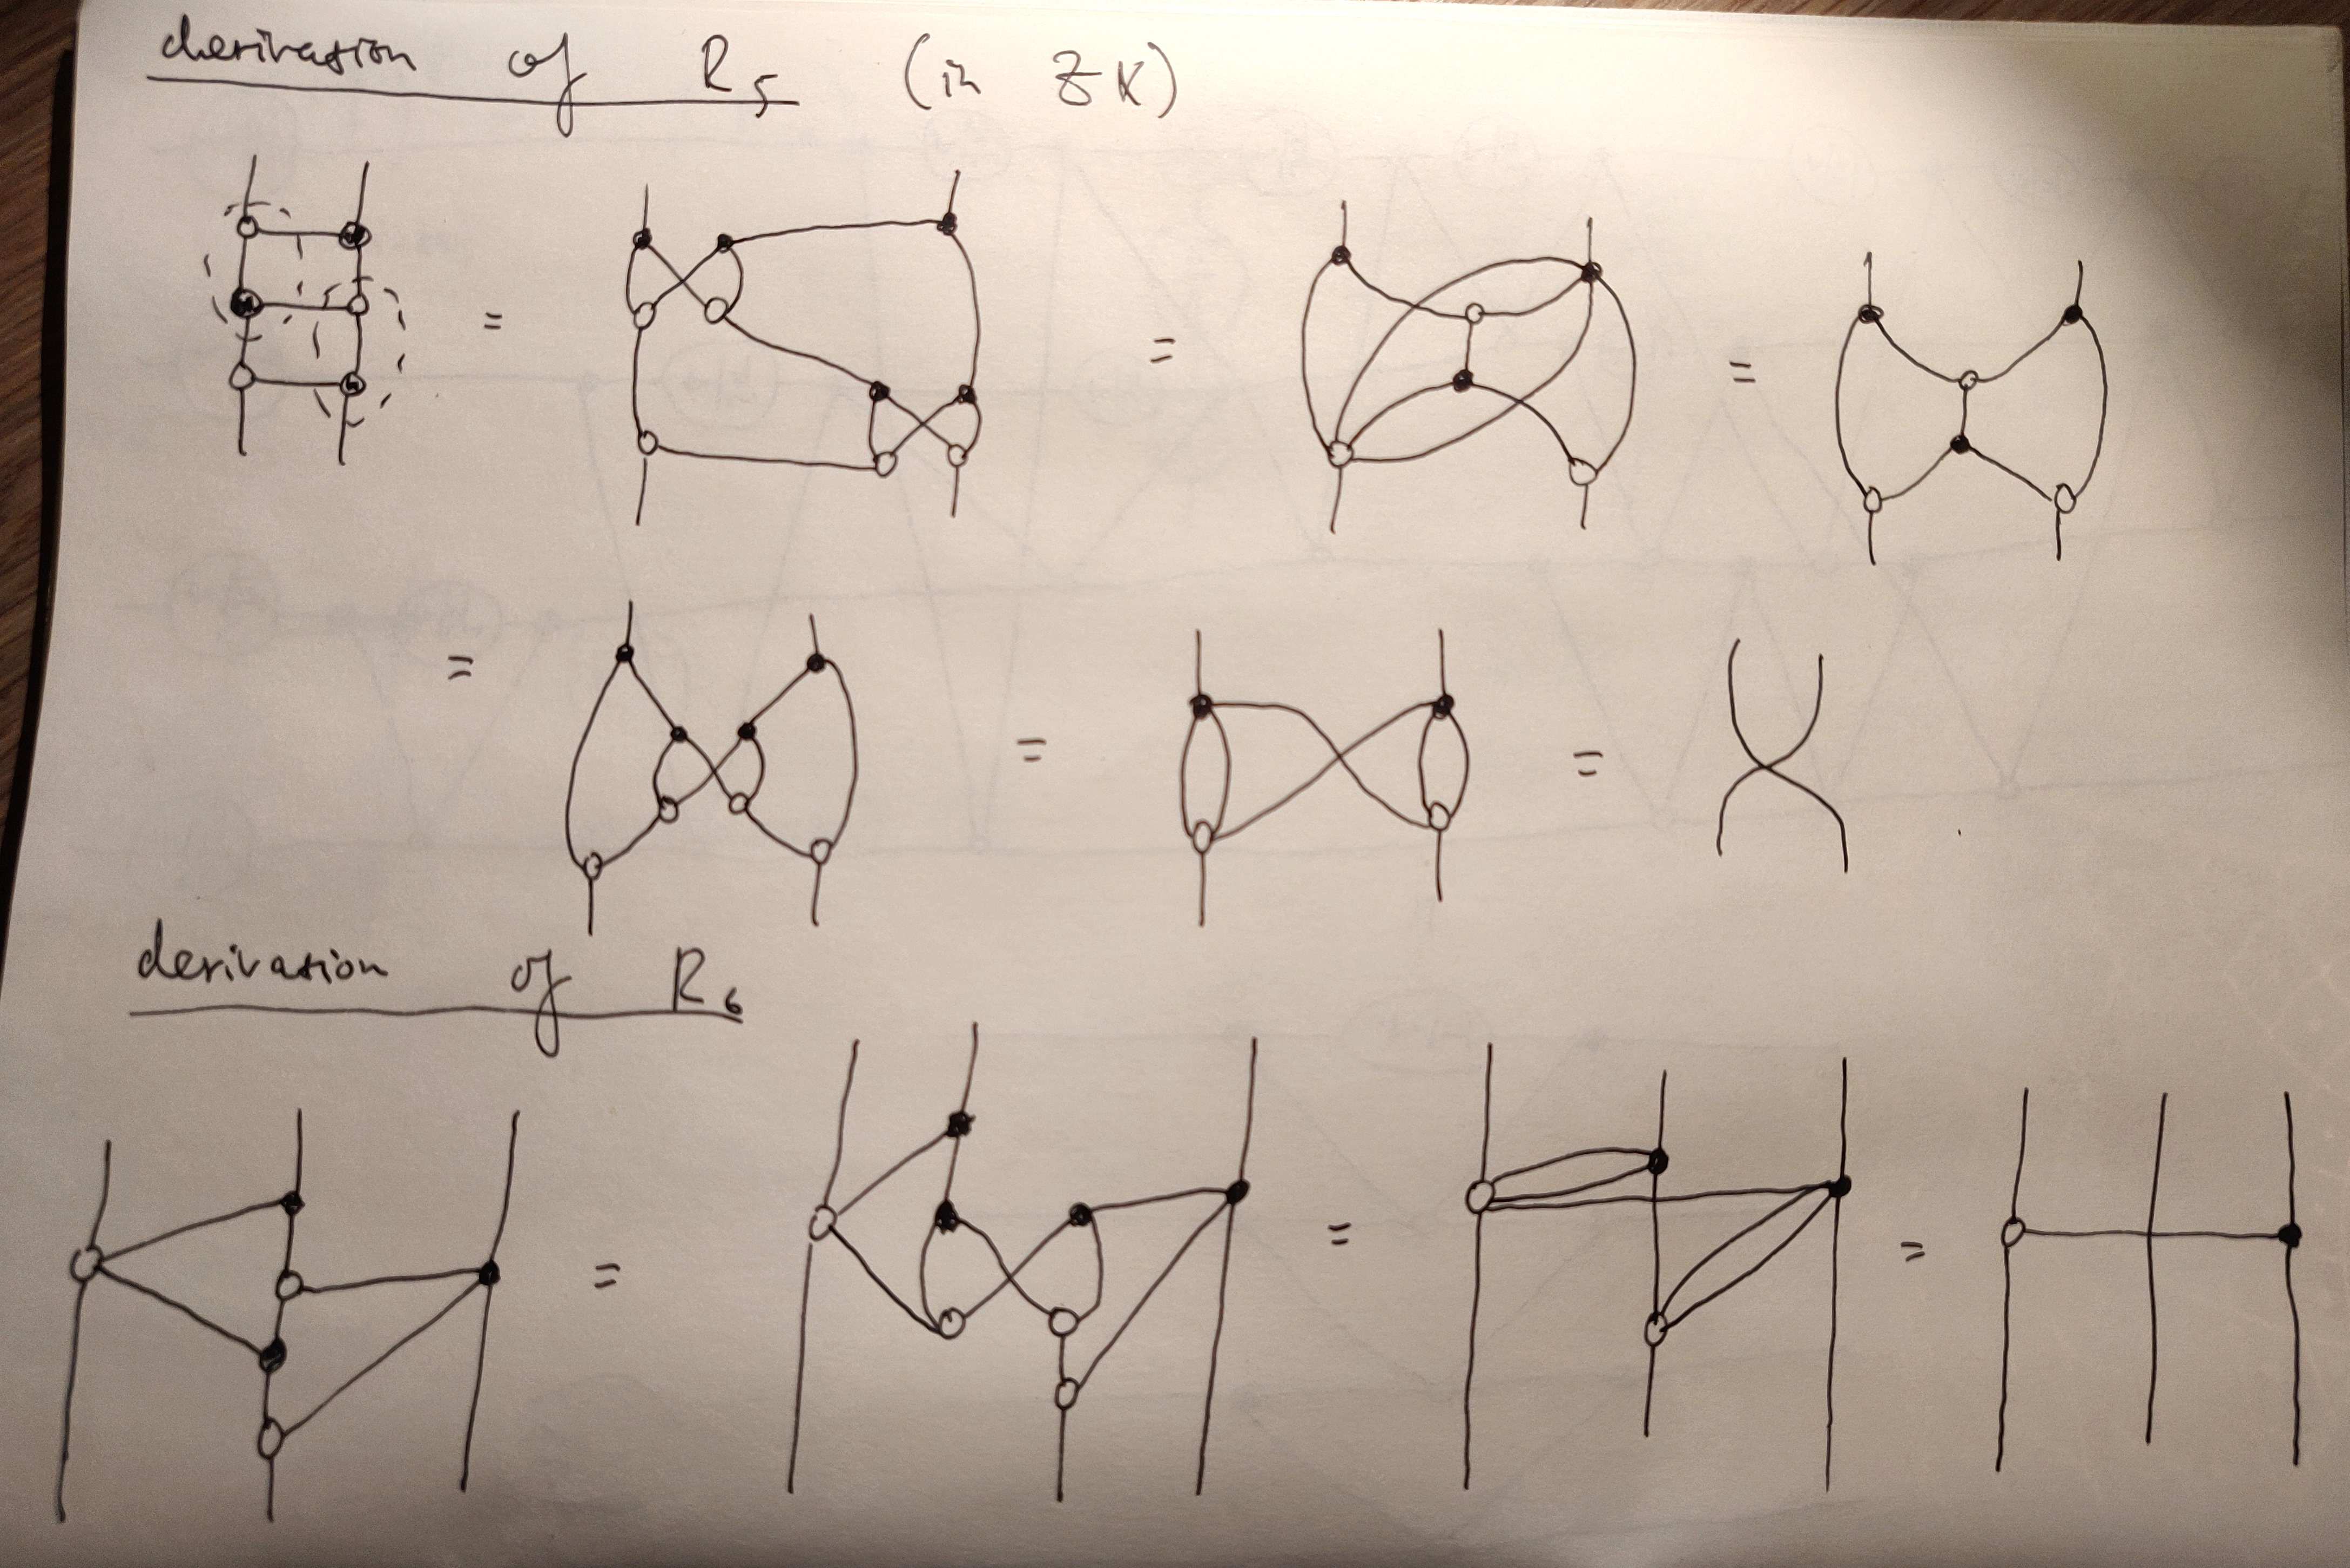
\includegraphics[width=10cm]{R5-R6}
\centering
\end{figure}
\end{frame}

\begin{frame}{Commutation rules}

\begin{figure}
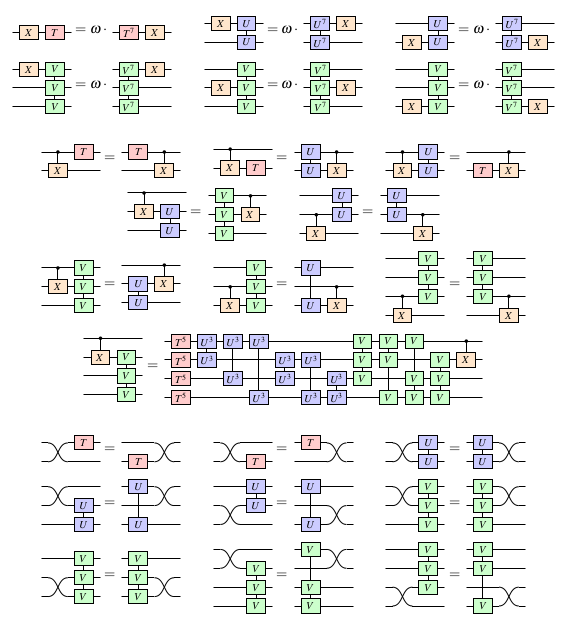
\includegraphics[width=7cm]{commutation-rules}
\centering
\end{figure}
\end{frame}

\section{Normal forms}

\begin{frame}{Normal forms}

\begin{figure}
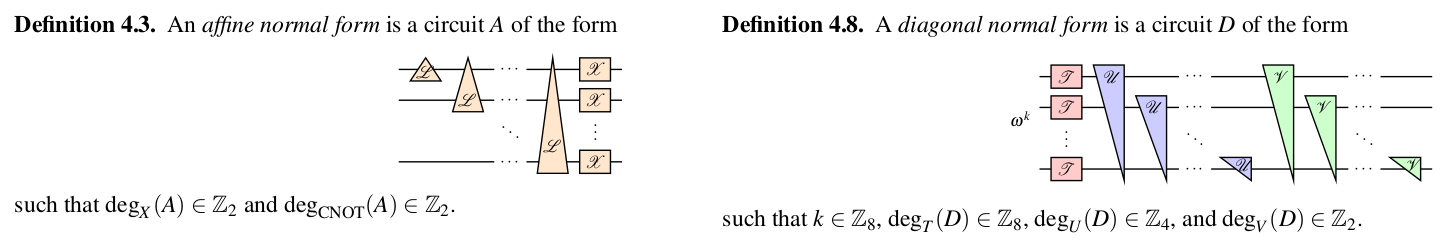
\includegraphics[width=11cm]{normal-forms}
\centering
\end{figure}
\begin{itemize}
\item Degrees in the normal forms reflect the degree reduction rules.
\item Every affine circuit admits a unique normal form (Lafont, 2003).
\item Every diagonal circuit admits a normal form (Lemma 5.3.)
\item Every CNOT-dihedral circuit $C$ admits a normal form $C=DA$, where $D$ is a diagonal circuit in normal form and $A$ is an affine circuit in normal form.
\end{itemize}
\end{frame}

\section{Phase polynomials and uniqueness}

\begin{frame}{Phase polynomials}

Action of a diagonal gate:
$$ D \ket{x} = \omega^{p_D(x)}\ket{x}, \quad p_D: \mathbb{Z}_2^n \rightarrow \mathbb{Z}_8 ,$$
%$$ p_D(x) = \sum_{i=1}^k a_i g_i(x) .$$
%where $a_i \in \mathbb{Z}_8$ and $g_i:\mathbb{Z}_2^n \rightarrow \mathbb{Z}_2$ are terms on at most $n$ variables.
$$ \omega^k \ket{x} = \omega^k \ket{x} $$
$$ T^k \ket{x_1} = \omega^{kx_1}\ket{x_1}$$
$$ U^k \ket{x_1x_2} = \omega^{k(x_1\oplus x_2)}\ket{x_1x_2}$$
$$ V^k \ket{x_1x_2x_3} = \omega^{k(x_1\oplus x_2 \oplus x_3)}\ket{x_1x_2x_3}$$
Therefore for $D$ in normal form we have
$$ p_D(x) = a_0 + \sum_i a_i x_i + \sum_{i<j}b_{ij} (x_i \oplus x_j) + \sum_{i<j<k}c_{ijk} (x_i \oplus x_j \oplus x_k)$$
Where $a_i \in \mathbb{Z}_8$, $b_{ij} \in \mathbb{Z}_4$, $c_{ijk} \in \mathbb{Z}_2$ (from the bounds on $deg_X(D)$ for $X=T,U,V$ obtained in normal form).

\end{frame}

\begin{frame}{Uniqueness}
Suppose $D$ and $D'$ are distinct diagonal normal forms, we want to show that $\exists y \in \mathbb{Z}^2$ such that $D\ket{y} \neq D'\ket{y}$.\\

By construction $p_D(x) \neq p_{D'}(x)$ as polynomials. However this does not mean that $\exists y \in \mathbb{Z}_2^n$ s.t. $p_D(y) \neq p_{D'}(y)$.\\

Counterexample: $4x_1 + 4x_2 + 4(x_1 \oplus x_2) = 0$ mod $8$ for any $x_1, x_2 \in \mathbb{Z}_2$\\

The existence of such a $y$ comes from the bounds on the coefficients $a_i$, $b_{ij}$ and $c_{ijk}$.

Construct a multilinear polynomial $q : \mathbb{Z}_8^n \rightarrow \mathbb{Z}_8$ such that $p_D(y)- p_{D'}(y) = q(y)$ $\forall y \in \mathbb{Z}_2^n$.

Do this by translating from mod $2$ to mod $8$:
$$ x_i \oplus x_j = x_i + x_j -2x_ix_j $$
$$ x_i \oplus x_j \oplus x_k = x_i + x_j + x_k -2x_ix_j -2x_ix_k -2x_jx_k + 4x_ix_jx_k$$

Then $p_D(x) - p_{D'}(x) \neq 0$ $\implies q(x) \neq 0$, because of the bounds on $a_i$, $b_{ij}$ and $c_{ijk}$. Pick a non-zero term $d x_{i_1} \dots x_{i_k}$ in $q(x)$ and let $y$ have $1$'s in $i_j$th positions and zero everywhere else. Then $q(y) = d \neq 0$ and so $D\ket{y} \neq D' \ket{y}$.
\end{frame}

\section{Open questions}
\begin{frame}{Open questions}
	\begin{itemize}
		\item Interaction between ZX and CNOT-dihedral rules (rule 13?).
		\item Phase polynomials representations for graph rewriting.
		\item Algebraic vs combinatorial description: the paper doesn't contain an algorithm for normalizing CNOT-dihedral circuits, it uses the properties of the ambient symmetric monoidal structure non-constructively. What would be a rewrite system?
		\item Complexity of CNOT-dihedral circuits: word problem for CNOT-dihedral circuits? Classical simulation of the normal form?
	\end{itemize}
\end{frame}


\end{document}
